\documentclass[aspectratio=169, t, 8pt]{beamer}

%------configurando acentos-----------
\usepackage[utf8]{inputenc}
\usepackage[brazil]{babel}

\usepackage{graphicx}

%-------Estilos Beamer---------------
\usetheme{metropolis}
%\usecolortheme{crane}
%\usefonttheme{serif}
\linespread{1.2}

% Personalização de Cores (Exemplo: Minimal Teal)
% Cores Base
\definecolor{BgCanvas}{HTML}{F9F9FB}      % Off-white muito suave
\definecolor{MainText}{HTML}{2B2D42}      % Grafite escuro para alta legibilidade
\definecolor{PrimaryAccent}{HTML}{4A6FA5} % Az
\definecolor{SunCoastFg}{HTML}{F2A154}
% --- CONFIGURAÇÕES DE TEMA BEAMER ---
%\usetheme{metropolis}

\setbeamertemplate{itemize item}{\textcolor{MainText}{$\bullet$}}
\setbeamertemplate{itemize subitem}{\textcolor{MainText}{\scriptsize$\circ$}}
\setbeamertemplate{itemize 3rditem}{\textcolor{MainText}{\tiny$\blacksquare$}}

\setbeamercolor{background canvas}{bg=BgCanvas}
\setbeamercolor{normal text}{fg=MainText}
\setbeamercolor{frametitle}{bg=SunCoastFg, fg=BgCanvas}
\setbeamercolor{title}{fg=MainText}
\setbeamercolor{subtitle}{fg=PrimaryAccent}
\setbeamercolor{structure}{fg=PrimaryAccent}

% Remove a linha amarela padrão do Metropolis sob o título
\setbeamertemplate{title separator}{}
\setbeamertemplate{progress bar in section page}{}


%--------Dados do Documento
\title{Matemática: Lista de Exercícios}
\author{prof. Eduardo}
\institute{Pré-Universitário Oficina do Saber / UFF}
\date{\today}


%-------- Pacotes Matemática -------------
\usepackage{amsmath}
\usepackage{amsthm}
\usepackage{amsfonts}
\usepackage{amssymb}
\usepackage{xfrac}
\usepackage{thmtools}

%-------- Configuração Listas---------
% \usepackage{enumitem}
\usepackage[inline]{enumitem}

\setcounter{tocdepth}{2}

\newcounter{questaovest}
\newcommand{\vest}[1]{\stepcounter{questaovest}\item[\textbf{Questão \arabic{questaovest}} (#1):]}
\setlist[enumerate]{
    align=left,
    leftmargin=1.8em,
    itemindent=1.8em
    }

\setlist[enumerate,2]{
    label=\alph*.,
    font=\bfseries,
    itemsep=0.1pt,
    labelsep=0em,
    parsep=0pt,
    leftmargin=0em,
    }

%------------- Atalho para imagens ------------
\graphicspath{{../../src/img/semana04/}}


\begin{document}

\begin{frame} %capa
        \vspace*{\fill}
            
            \begin{columns}[c]
                \begin{column}{0.5\textwidth}
                    {\usebeamerfont{title}\usebeamercolor[fg]{title}\inserttitle}\vspace{0.2cm}
                    
                    {\usebeamerfont{subtitle}\usebeamercolor[fg]{subtitle}\insertsubtitle}\vspace{0.5cm}

                {\usebeamerfont{author}\insertauthor}\vspace{0.3cm}

                {\usebeamerfont{institute}\insertinstitute}\vspace{0.3cm}

                {\usebeamerfont{date}\insertdate}
            \end{column}
            
            
            \begin{column}{0.4\textwidth}
                \centering
                
\includegraphics[width=0.4\textwidth]{../logo_ofSaber.png}

                \vspace{.4cm}
                \vspace*{\fill}
        \begin{columns}[c]
            \begin{column}{.5\textwidth}
                \centering
\includegraphics[width=.5\textwidth]{../Proex02c.png}
            \end{column}
            \begin{column}{.5\textwidth}
                \centering
\includegraphics[width=0.4\textwidth]{../Logo_UFF.png}
            \end{column}
        \end{columns}
        \vspace*{\fill}
            \end{column}
        \end{columns}
    \vspace*{\fill}
    \end{frame}
    
        % {
        %     \usebackgroundtemplate{
        %     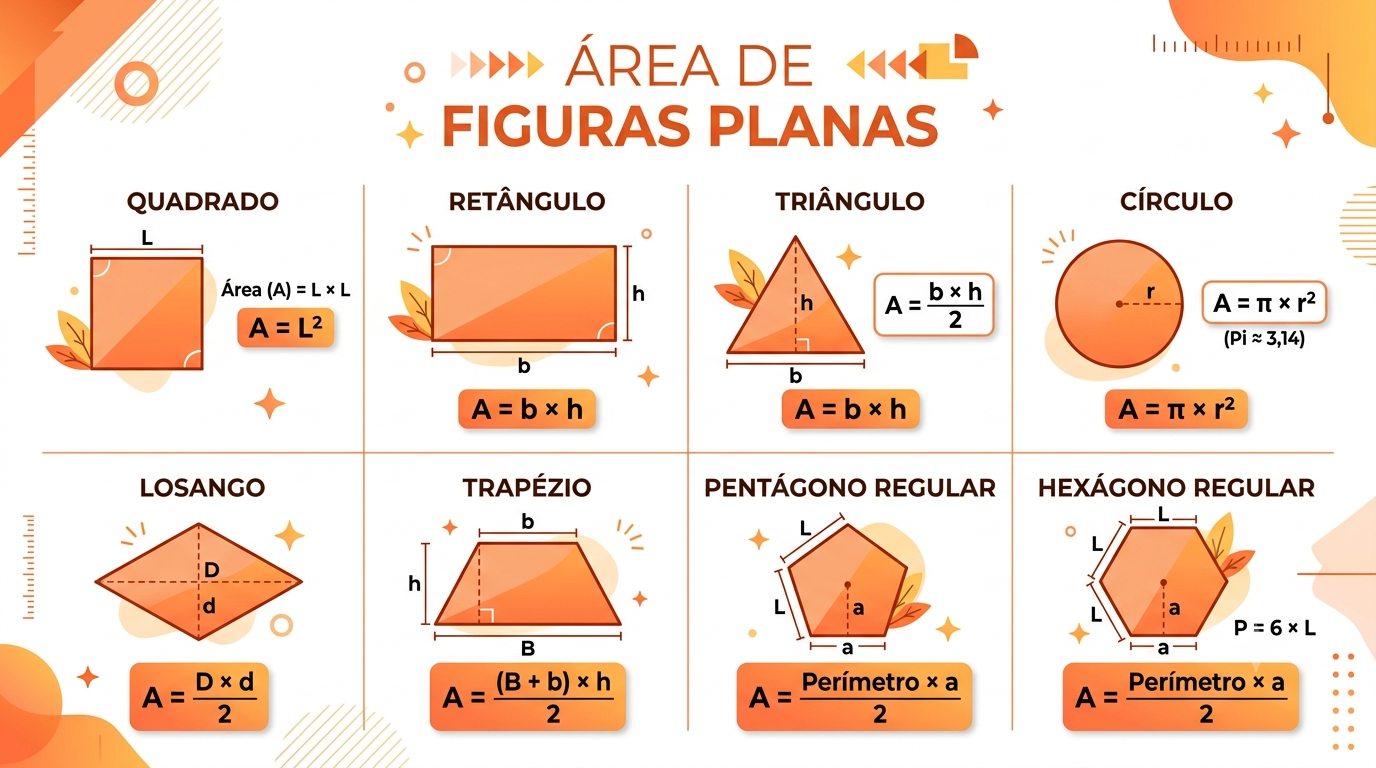
\includegraphics[width=\paperwidth]{slide_02_contracapa.png}}
        %     \begin{frame}[plain]                
        %     \end{frame}
        % }


    \begin{frame} %Questão 01-B
        \frametitle{Combinatória}
        \vspace{-1.2em}
        \begin{enumerate}
            \begin{columns}
                \begin{column}{.9\textwidth}
                    \vest{ENEM-2024} Para abrir a porta de uma empresa, cada funcionário deve cadastrar uma senha utilizando um teclado alfanumérico como o representado na figura.
                    
                    Por exemplo: a tecla que contém o número 2 traz as letras correlacionadas A, B e C. Cada toque nessa tecla mostra, sequencialmente, os seguintes caracteres: 2, A, B e C. Para os próximos toques, essa sequência se repete. As demais teclas funcionam da mesma maneira.

                    \begin{columns}[T, totalwidth=.9\textwidth]                       
                        \begin{column}{0.4\textwidth}
                                \begin{figure}[H]
                                    \centering
                                    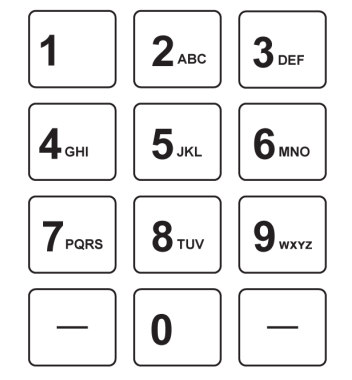
\includegraphics[width=.75\textwidth]{lista_q01.png}
                                \end{figure}
                        \end{column}
                        \begin{column}{.6\textwidth}
                            As senhas a serem cadastradas pelos funcionários devem conter 5 caracteres, sendo 2 algarismos distintos seguidos de 3 letras diferentes, nessa ordem. Um funcionário irá cadastrar a sua primeira senha, podendo escolher entre as teclas que apresentam os números 1, 2, 5, 7 e 0 e as respectivas letras correlacionadas, quando houver.

                            O número de possibilidades diferentes que esse funcionário tem para cadastrar sua senha é

                            \vspace{1em}
                            \centering
                            \begin{minipage}{0.9\textwidth}
                                \begin{enumerate*}[itemjoin={\hfill}]
                                    \item $11.520$
                                    \item $14.400$
                                    \item $18.000$
                                    \item $312.000$
                                    \item $390.000$
                                    %gabarito: B
                                \end{enumerate*}
                            \end{minipage}
                            \end{column}

                    \end{columns}

                \end{column}
            \end{columns}
        \end{enumerate}
    \end{frame}

    \begin{frame} %Questão 02-B
        \frametitle{Geometria}
        \begin{columns}
            \begin{column}{.9\textwidth}
                \begin{enumerate}
                    \vest{ENEM-2019} No trapézio isósceles mostrado na figura a seguir, $M$ é o ponto médio do segmento $BC$, e os pontos $P$ e $Q$ são obtidos dividindo o segmento $AD$ em três partes iguais.
                    
                    Pelos pontos $B, M, C, P$ e $Q$ são traçados segmentos de reta, determinando cinco triângulos internos ao trapézio, conforme a figura. A razão entre $BC$ e $AD$ que determina áreas iguais para os cinco triângulos mostrados na figura é
                    \vspace{1.2em}
                    \begin{columns}[T, totalwidth=.8\textwidth]
                        \begin{column}{.4\textwidth}
                            \begin{figure}
                                \centering
                                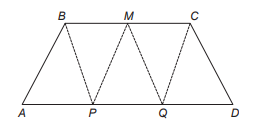
\includegraphics[width=0.9\textwidth]{lista_q02.png}
                            \end{figure}
                        \end{column}
                        \begin{column}{.55\textwidth}
                            \begin{enumerate*}[itemjoin={\hfill}]
                                \item $\displaystyle \frac{1}{3}$
                                \item $\displaystyle \frac{2}{3}$
                                \item $\displaystyle \frac{2}{5}$
                                \item $\displaystyle \frac{3}{5}$
                                \item $\displaystyle \frac{5}{6}$
                                %gabarito B
                            \end{enumerate*}
                        \end{column}
                    \end{columns}
                \end{enumerate}
            \end{column}
        \end{columns}
    \end{frame}

    \begin{frame} %Questão 03-B
        \frametitle{Função}
        \begin{columns}[T, totalwidth=.9\textwidth]
            \begin{column}{\textwidth}
                \begin{enumerate}
                    \vest{FGV-2012} Os gráficos abaixo representam as funções receita mensal $R(x)$ e custo mensal $C(x)$ de um produto fabricado por uma empresa, em que $x$ é a quantidade produzida e vendida. Qual o lucro obtido ao se produzir e vender 1350 unidades por mês?
                    \begin{columns}[T, totalwidth=.9\textwidth]
                        \begin{column}{.6\textwidth}
                            \centering
                            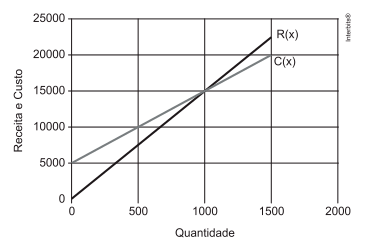
\includegraphics[width=.9\textwidth]{lista_q03.png}
                        \end{column}
                        \begin{column}{.35\textwidth}
                            \begin{enumerate}
                                \item 1740
                                \item 1750
                                \item 1760
                                \item 1770
                                \item 1780
                                %gabarito: B
                            \end{enumerate}
                        \end{column}
                    \end{columns}
                \end{enumerate}
            \end{column}
        \end{columns}
    \end{frame}
    
    \begin{frame} %Questão 04-D
        \frametitle{Geometria}
        \begin{columns}[T, totalwidth=.9\textwidth]
            \begin{column}{\textwidth}
                \begin{enumerate}
                    \vest{UNESP-1990} Uma gangorra é formada por uma haste rígida AB, apoiada sobre uma mureta de concreto no ponto C, como na figura. Quando a extremidade B da haste toca o chão, a altura da extremidade A em relação ao chão é:

                    \begin{columns}[T, totalwidth=.9\textwidth]
                        \begin{column}{.4\textwidth}
                            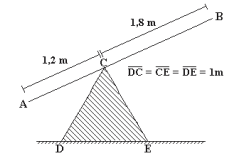
\includegraphics[width=.9\textwidth]{lista_q04.png}
                        \end{column}
                        \begin{column}{.55\textwidth}
                            \begin{enumerate*}[itemjoin={\hfill}]
                                \item $\displaystyle \sqrt{3}\text{ m}$
                                \item $\displaystyle \frac{3}{\sqrt{3}}\text{ m}$
                                \item $\displaystyle \frac{(6\sqrt{3})}{5}\text{ m}$
                                \item  $\displaystyle \frac{(5\sqrt{3})}{6}\text{ m}$
                                \item $\displaystyle 2\sqrt{2}\text{ m}$
                                %gabarito D
                            \end{enumerate*}
                        \end{column}
                    \end{columns}
                \end{enumerate}
            \end{column}
        \end{columns}
    \end{frame}

    \begin{frame} %Questão 05-C
        \frametitle{Geometria}
        \begin{columns}[T, totalwidth=.9\textwidth]
            \begin{column}{\textwidth}
                \begin{enumerate}
                    \vest{EEAR-2017} No quadrilátero $ABCD$, o valor de $y-x$ é igual a:
                    \vspace{1.2 em}
                    \begin{columns}[T, totalwidth=.9\textwidth]
                        \begin{column}{.4\textwidth}
                            \centering
                            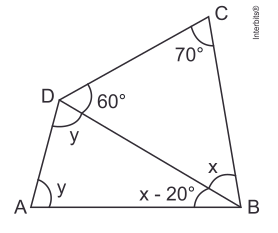
\includegraphics[width=\textwidth]{lista_q05.png}
                        \end{column}
                        \begin{column}{.4\textwidth}
                            \begin{enumerate*}[itemjoin={\hfill}]
                                \item $2x$
                                \item $2y$
                                \item $\displaystyle \frac{x}{2}$
                                \item $\displaystyle \frac{y}{2}$
                                %gabarito C
                            \end{enumerate*}
                        \end{column}
                    \end{columns}
                \end{enumerate}
            \end{column}
        \end{columns}
    \end{frame}

    \begin{frame} %Questãao 06-B
        \frametitle{Geometria}
        \begin{columns}[T, totalwidth=.9\textwidth]
            \begin{column}{\textwidth}
                \begin{enumerate}
                    \vest{PUCR-RS/2013} Um desafio matemático construído pelos alunos do Curso de Matemática tem as peças no formato de um cone. A figura abaixo representa a planificação de uma das peças construídas.
                    \vspace{0.5em}
                    \begin{columns}[T, totalwidth=.9\textwidth]
                        \begin{column}{.4\textwidth}
                            \centering
                            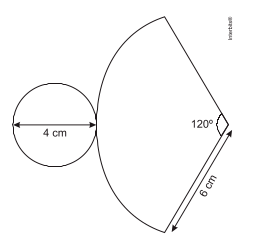
\includegraphics[width=.9\textwidth]{lista_q06.png}
                        \end{column}
                        \begin{column}{.4\textwidth}
                            A área total dessa peça é de \underline{\hspace{.5cm}} $\text{cm}^2$

                            \vspace{1em}
                            
                            \begin{enumerate*}[itemjoin={\hfill}]
                                \item $10\pi$
                                \item $16\pi$
                                \item $20\pi$
                                \item $28\pi$
                                \item $40\pi$
                                % gabarito B 
                            \end{enumerate*}
                        \end{column}
                    \end{columns}
                \end{enumerate}
            \end{column}
        \end{columns}
    \end{frame}

\end{document}